\documentclass[conference, onecolumn]{IEEEtran}
% \usepackage{cite}
% \usepackage{amsfonts}
\usepackage{amssymb}
\usepackage{amsmath}
\usepackage{filecontents}
\usepackage{url}
\usepackage{bm}
 \usepackage[square,sort,comma,numbers]{natbib}
%  \usepackage{caption}
% \usepackage{subcaption}

\usepackage{graphicx}
\usepackage{subfigure}
% \usepackage{caption}
% \usepackage{subcaption}

\usepackage{wrapfig}

% \ifCLASSINFOpdf
%  \usepackage[pdftex]{graphicx}
% \else
%  \usepackage[dvips]{graphicx}
% \fi




% correct bad hyphenation here
\hyphenation{op-tical net-works semi-conduc-tor}

\renewcommand{\citedash}{--}

\DeclareMathOperator*{\argmax}{arg\,max}

\begin{document}
%
% paper title
% can use linebreaks \\ within to get better formatting as desired
\title{Entropy Minimization Based Symbol Rate\\ 
and Symbol Timing Estimation}


% author names and affiliations
% use a multiple column layout for up to three different
% affiliations
\author{


%\IEEEauthorblockN{Jean-Fran\c{c}ois Bousquet, IEEE Member}
% \IEEEauthorblockA{Electrical and Computer Engineering, Dalhousie University, Halifax, Nova Scotia\\ 
%email: jbousquet@dal.ca}

\IEEEauthorblockN{Xiao Liu and Jean-Fran\c{c}ois Bousquet}
\IEEEauthorblockA{Department of Electrical and Computer Engineering, Dalhousie University,
% \\1340 Barrington St
% Halifax, NS, B3J 1Z1, Canada\\ 
Halifax, Canada\\
Email: x.liu@dal.ca
}
}


% make the title area
\maketitle

\IEEEpeerreviewmaketitle


\section{Background}


In a digital receiver for underwater acoustic communication, to achieve maximum noise immunity, the decision samples should be taken at the instants of maximum eye opening. 
Due to the channel complexity and the relative mobility, the exact symbol clock is unknown in the receiver.  
So the receiver must contain a synchronization device which makes an estimate of the symbol rate and symbol timing, 
then recovers the data with the correct down sampling clock for decision making \cite{mengali1997synchronization}.  
In this paper, an entropy minimization based synchronization criterion is proposed for this purpose.
% It is an alternative synchronization scheme. 
% and it is a good complement for Maximum Likelihood (ML) based schemes,
Especially in complex channel environments, it can provide improved synchronization performance in combination with Maximum Likelihood (ML) based schemes.

\section{Entropy minimization based synchronization}

% Fig. \ref{fig:timing_freq} is the eye diagrams for a BPSK signal when the symbol rate has 1\% error and no error. 
The eye diagram for a pulse shaped PSK signal with a 1\% symbol rate error is shown in Fig. \ref{fig:timing_freq}. 
Similarly, Fig.\ref{fig:timing_phase} shows an eye diagram but with a perfect timing recovery. 
Clearly, it is impossible to obtain an open eye without a correct estimate of the symbol rate.
Traditional ML based symbol rate estimation schemes are essential to find out the periodicity of the signal energy \cite{Mosquera2008},
as a result, the information of waveform distribution is neglected.
However, Fig. \ref{fig:timing_phase} provides us an intuitive impression that when the correct symbol rate is obtained, the eye diagram has a well-organized pattern. 
It has less ``randomness'' compared to Fig. \ref{fig:timing_freq} where the symbol rate is incorrect.

\begin{figure}[htbp]
  \centering
    \subfigure[Symbol rate error induced moving eye diagram with 1\% symbol rate error]{
    \label{fig:timing_freq} 
    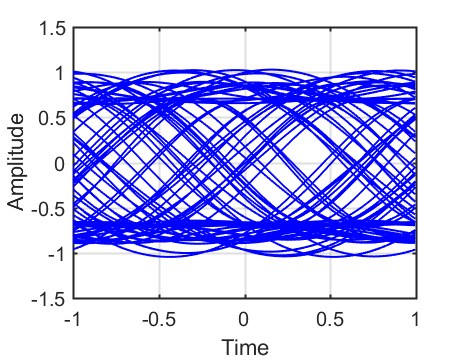
\includegraphics[width=2.5in]{sym_rate_wrong.png}}
  \hspace{0.2in} % 两图间距
  \subfigure[Eye diagram after ideal symbol recovery]{
    \label{fig:timing_phase} 
    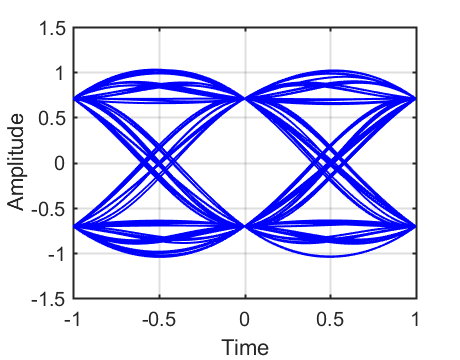
\includegraphics[width=2.5in]{sym_rate_right.png}}
  
    \caption{Eye diagrams of a bandlimited PSK signal. }
    \label{fig:timing} %% 总 label
\end{figure}


This phenomenon suggests that the randomness can be employed as an alternative criterion by which the symbol rate can be estimated.
In addition, the optimal symbol timing can be found in Fig \ref{fig:timing_phase} in a similar way. 
The randomness comes to a minimum in the middle of the eye diagram, 
so the the randomness can also be treated as a criterion for symbol timing estimation.
% This application can be demonstrated more clearly with PAM of QAM modulation.
Also, the using of randomness measurement is attractive because it can be easily expanded to carrier frequency recovery, as will be demonstrated in a future paper.

To quantitatively measure the randomness, the concept of entropy is employed.
The Shannon entropy \cite{Shannon1948} is a fundamental concept in information theory and it is a measure of the randomness of a signal.
The Shannon entropy \(H\) of a one-dimensional discrete signal can be expressed as
\begin{equation}
H =  - \sum\limits_{i = 1}^n {{p_i}\log {p_i}},
\label{eq:entropy}
\end{equation}
where \(p_i\) is the probability of samples falling into the \textit{i}-th amplitude bin.

The innovation of this paper is to estimate the symbol rate and symbol timing using the entropy minimization criterion.
As a preliminary study, the entropy minimum is found by global searching,
which means the entropy is calculated through all the possible symbol rate and timing ranges, such that a global minimum can be searched out.
This can be done by parallel computation to accelerate the speed.
More practical algorithms will be discussed in the future.
% The  
% To avoid the local minimum, the signal energy cannot be discarded completely.

\section{Simulation and evaluation}

The entropy of the BPSK signal mentioned above is plotted as a function of the symbol rate and symbol timing error in Fig. \ref{fig:entropy}.
It shows that there is a global minimum for both figures when the error is equal to zero.
It proves that the entropy minimization is a feasible criterion for both symbol rate and symbol timing estimation.

\begin{figure}[htbp]
  \centering
    \subfigure[Entropy as a function of symbol rate estimation error]{
    \label{fig:etp_rate} 
    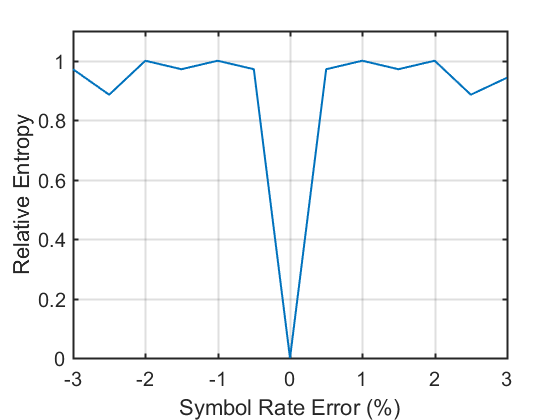
\includegraphics[width=2.5in]{etp_rate.png}}
  \hspace{0.2in} % 两图间距
  \subfigure[Entropy as a function of symbol timing estimation error]{
    \label{fig:etp_timing} 
    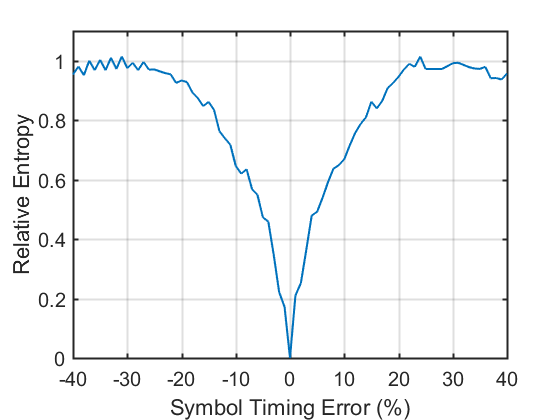
\includegraphics[width=2.5in]{etp_timing.png}}
  
    \caption{Entropy minimization based synchronization}
    \label{fig:entropy} %% 总 label
\end{figure}

Moreover, the entropy minimization detector can be easily modified to a clock-aided carrier frequency offset detector \cite{Pedzisz2006}.
The entropy reaches minimum when the constellation stops rotating. 
It means that only after symbol timing and carrier frequency recovery, 
the entropy of the received data will come to a global entropy minimum.
It gives us an all-in-one principle for synchronization.
% Note that in Fig. \ref{fig:etp_timing}, the local minimum on each side may introduce false estimate, 
% but it can be avoided with the help of ML based symbol timing schemes \cite{mengali1997synchronization}.
Also the comparison with the standard cyclostationarity based symbol rate \cite{Wu2012} and symbol timing methods~\cite{Wang2004a} will be given for realistic underwater propagation conditions, 
that are subject to multipath arrival as well as Doppler. 
For this purpose, the synchronization algorithm will also be applied to real measurement data. 
% This demonstrates the advantage of 





\vspace{-0.2cm}
\bibliographystyle{IEEEbib}
% \bibliographystyle{plain}
\bibliography{Mendeley}

\end{document}